%%%%%%%%%%%%%%%%%%%%%%%%%%%%%%%%%%%%%%%%%%%%%%%%%%%%%%%%%%%%%%%%%%%%%%%%%%%%%%%%
\section{About Continuous Integration}
{   
	\usebackgroundtemplate{
		\vbox to \paperheight{\vfil\hbox to \paperwidth{\hfil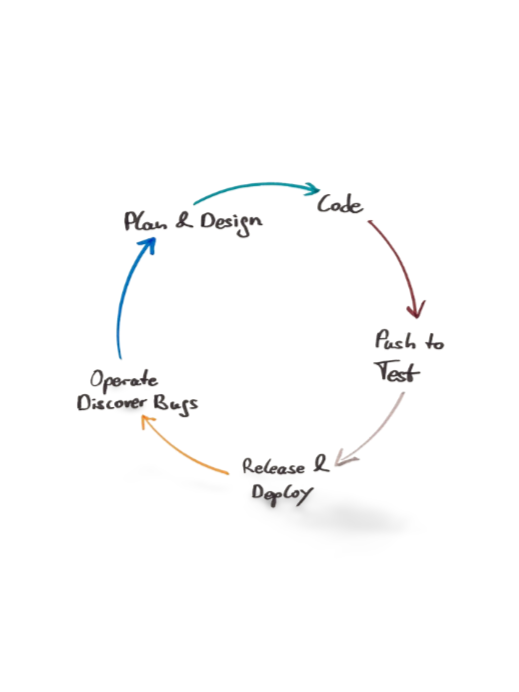
\includegraphics[height=\paperheight]{CI_enh.png}\hfil}\vfil}
		%https://www.flaticon.com/free-icon/decoration_2788716
		%<a href="https://www.flaticon.com/free-icons/decoration" title="decoration icons">Decoration icons created by Freepik - Flaticon</a>
		
	}
	\frame{
		\frametitle{The What \& Why}
		\begin{mdframed}[tikzsetting={draw=white,fill=white,fill opacity=0.8,
				line width=0pt},backgroundcolor=none,leftmargin=0,
			rightmargin=150,innertopmargin=4pt,roundcorner=10pt]
			\tableofcontents[currentsection,sections={1-6},hideothersubsections]
		\end{mdframed}
	}
}

%%%%%%%%%%%%%%%%%%%%%%%%%%%%%%%%%%%%%%%%%%%%%%%%%%%%%%%%%%%%%%%%%%%%%%%%%%%%%%%%
\begin{frame}
	\frametitle{The “Emotions”}
	\begin{columns}
		\begin{column}{0.5\textwidth}
			\centering 
			Idealized Software Development Cycle
			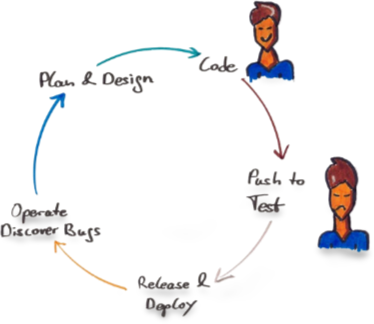
\includegraphics[width=0.8\textwidth]{CI_emotions_enh.png}
		\end{column}
		\begin{column}{0.5\textwidth}
			% A short introductory sentence (outside the list)
			What is Continuous Integration about?
			% The list with the *environment‑wide* overlay specification
			\begin{itemize}[<+->]
				\item We are passionate about coding \ldots
				\item But the TDD‑pill is hard to swallow
				\item Yet, needed for successful RSE projects.
			\end{itemize}
		\end{column}
	\end{columns}
\end{frame}

%%%%%%%%%%%%%%%%%%%%%%%%%%%%%%%%%%%%%%%%%%%%%%%%%%%%%%%%%%%%%%%%%%%%%%%%%%%%%%%%
\begin{frame}
	\frametitle{The “Background”}
	\begin{columns}
	    \begin{column}{0.5\textwidth}
			\centering 
			Idealized Software Development Cycle
			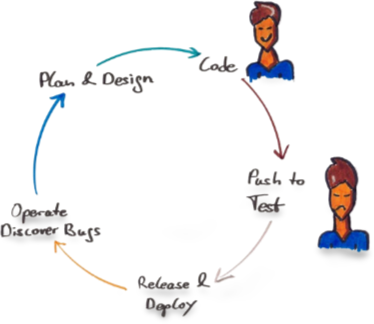
\includegraphics[width=0.8\textwidth]{CI_emotions_enh.png}
		\end{column}
		\begin{column}{0.5\textwidth}
			% A short introductory sentence (outside the list)
			We know \ldots
			% The list with the *environment‑wide* overlay specification
			\begin{itemize}[<+->]
				\item well tested  \ldots
				\item and actively maintained \ldots
			\end{itemize}
		    research software is used (and cited) more frequently
		    \pause
		    Also community building depends (in parts) on
		    \begin{itemize}[<+->]
		    	\item readable code
		    	\item and the knowing it is in good hands.
		    \end{itemize}
		\end{column}

	\end{columns}
\end{frame}

%%%%%%%%%%%%%%%%%%%%%%%%%%%%%%%%%%%%%%%%%%%%%%%%%%%%%%%%%%%%%%%%%%%%%%%%%%%%%%%%
\begin{frame}
	\frametitle{Which are the CI-Ingredients?}
	\begin{question}[What do you think?]
		{
		
\includegraphics[height=1.2em]{ingredients.jpg}
		What belongs to a CI Pipeline?
	}
	\end{question}
\end{frame}

%%%%%%%%%%%%%%%%%%%%%%%%%%%%%%%%%%%%%%%%%%%%%%%%%%%%%%%%%%%%%%%%%%%%%%%%%%%%%%%%
\begin{frame}
	\frametitle{Which are the CI-Constituents?}
	\begin{columns}
		\begin{column}{0.5\textwidth}
			\centering 
			Mandatory:
			\vfill
			\begin{itemize}[<+->]
				\item Version Control
				\item Package Management
				\item Automated Build Processes
				\item Automated Releases
			\end{itemize}
		\end{column}
		\begin{column}{0.5\textwidth}
			\centering
			Optional:
            \vfill

			\begin{itemize}[<+->]
			  \item Linting (Static Code Analysis)
			  \item for compiled languages: debug and release runs with difference compilers and settings, possibly checks for memory leaks.
			  \item Formatting (sometimes disliked)
			  \item Posting on Social Media
			\end{itemize}
		\end{column}	
	\end{columns}
\end{frame}

%%%%%%%%%%%%%%%%%%%%%%%%%%%%%%%%%%%%%%%%%%%%%%%%%%%%%%%%%%%%%%%%%%%%%%%%%%%%%%%%
\begin{frame}
	\frametitle{Our Current CI Options in RSE}
	\begin{columns}
		\begin{column}{0.4\textwidth}
			\centering 
			\only<1>{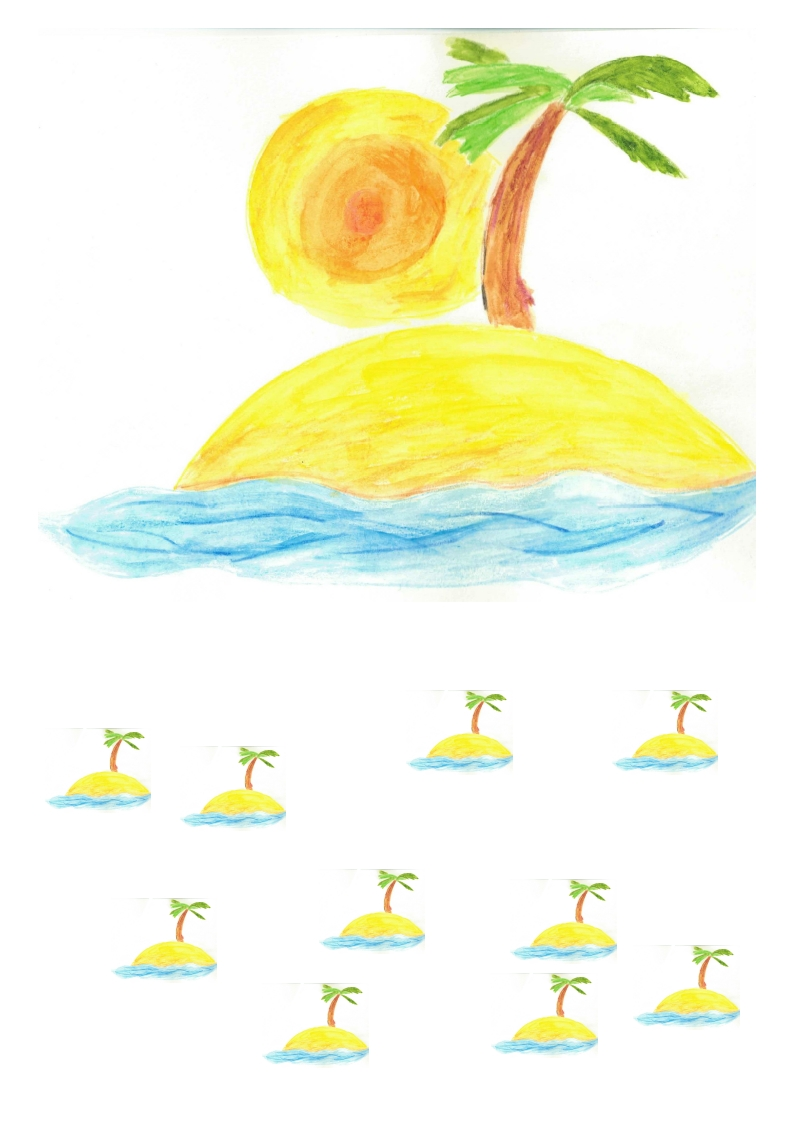
\includegraphics[width=0.8\textwidth]{Islands.jpg}}
			\only<2>{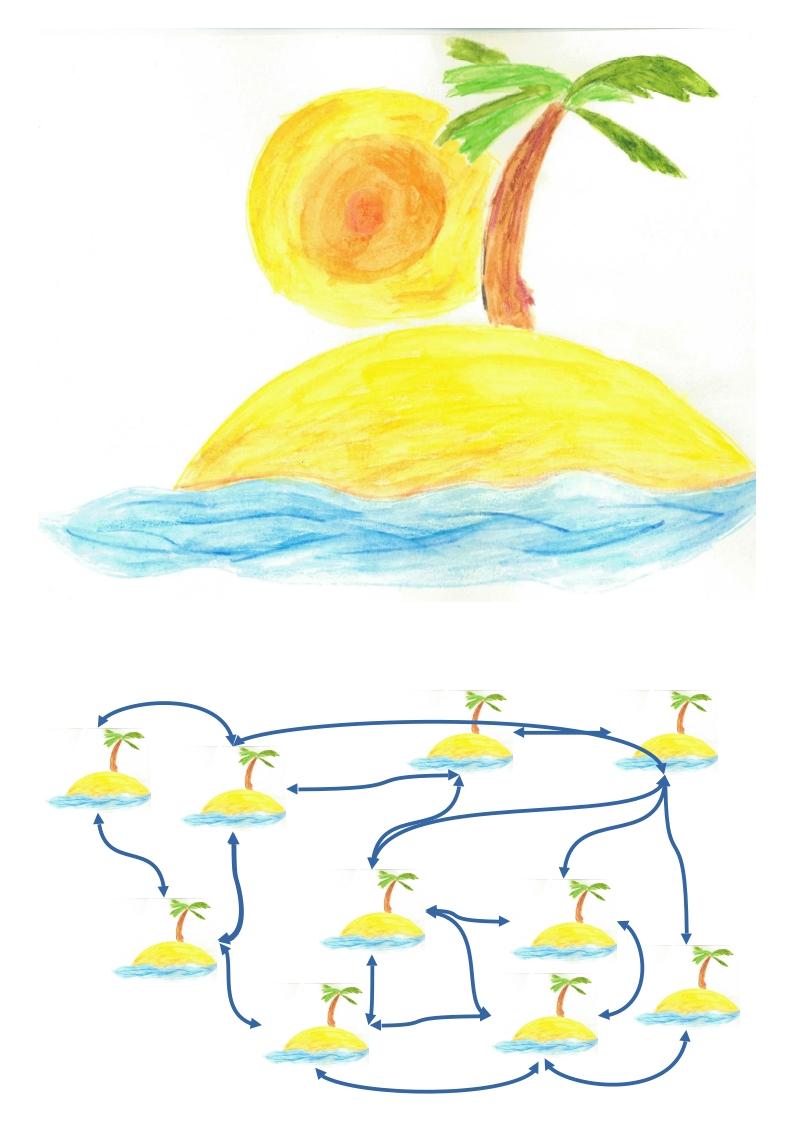
\includegraphics[width=0.8\textwidth]{Islands_connected.jpg}}
		\end{column}
		\begin{column}{0.6\textwidth}
			After cvs, svn, mecurial, etc. the RSE world settled for git -- close to 100 \% -- for source code management. Regarding CI, we have:
			\pause
			\begin{itemize}
				\item There is GitHub.com - the big beautiful island big enough for all, with all its cornucopia of features.
				\item Our institutions set on GitLab. Isolated. Good enough for interal projects.
				\only<3>{\item Perhaps, once ActivityPub is established for GitLab and Codeberg (Forgejo), we find ourselves in a different situation.}
			\end{itemize}
		\end{column}
	\end{columns}
\end{frame}

%%%%%%%%%%%%%%%%%%%%%%%%%%%%%%%%%%%%%%%%%%%%%%%%%%%%%%%%%%%%%%%%%%%%%%%%%%%%%%%%
\begin{frame}<handout:0>
	\frametitle{The Focus on GitHub}
	\begin{block}{This is why \ldots}
				\ldots we focus on GitHub, today. With bits of GitLab, too.\newline
		No Codeberg: The CI is with costs.\\
		This might change in future editions of this course.
	\end{block}
\end{frame}
	